\documentclass{article}
\usepackage{amsmath}
\usepackage{amssymb}
\usepackage{hyperref}
\usepackage{fancyhdr}
\usepackage{graphicx}
\usepackage{setspace}
\usepackage{caption}
\usepackage{wrapfig}
\usepackage{cancel}
\usepackage{pythonhighlight}
\usepackage{float}
\usepackage[a4paper, total={6in, 8in}]{geometry} 
\usepackage{mdframed}
\usepackage{tikz}


\graphicspath{C:\Users\cmark\OneDrive\Documents\Latex\PHSCS428\dp3}


\hypersetup{
    colorlinks=true,
    linkcolor=blue,
    urlcolor=cyan,
    citecolor = red
}

\pagestyle{fancy}
\renewcommand{\headrulewidth}{0.4pt}
\renewcommand{\footrulewidth}{0.4pt}
\setlength{\headheight}{18pt}
\setlength{\parindent}{12pt}

\lhead{\large{\bf Carter Garrett}} 
\chead{}
\rhead{\textsc{PHSCS 428, Data Project 3}} 
\lfoot{\today}
\cfoot{}
\rfoot{} 

\newmdtheoremenv{defi}{Definition}

\newcommand*\fancypants{\vcenter{\hbox{\includegraphics[width = 2.0em]{fp.png}}}}

\begin{document}

\section{Intro}
We experiment with making 'cuts' in different parameter spaces to determine actual members of the Pleiades cluster.    
We conducted the search and found upwards 130,000 targets within the solid angle.
Firstly, a total CMD was created.

\begin{figure}[H]
    \centering
    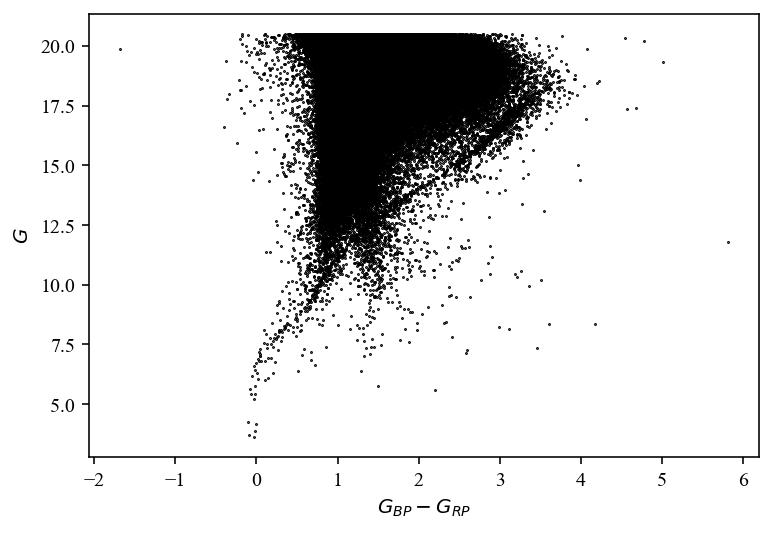
\includegraphics[scale = .5]{Figure 2025-02-08 230950 (0).png}
\end{figure}

The Pleiades appears to be the narrow thread of stars, underneath the blob that appears in the upper central region.

\section{Histogram}

We begin to make cuts in parameter space. 
Here are the histograms generated.

\begin{figure}[H]
    \centering
    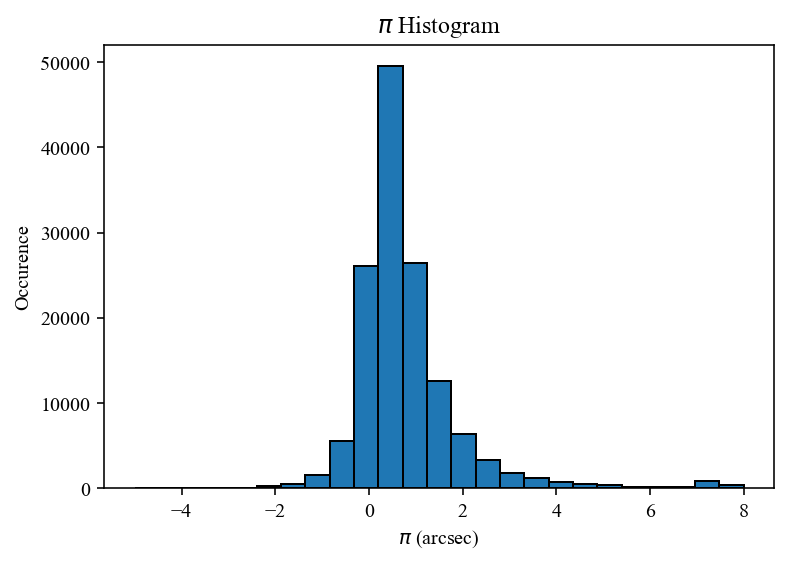
\includegraphics[scale = .5]{Figure 2025-02-08 230950 (1).png}
    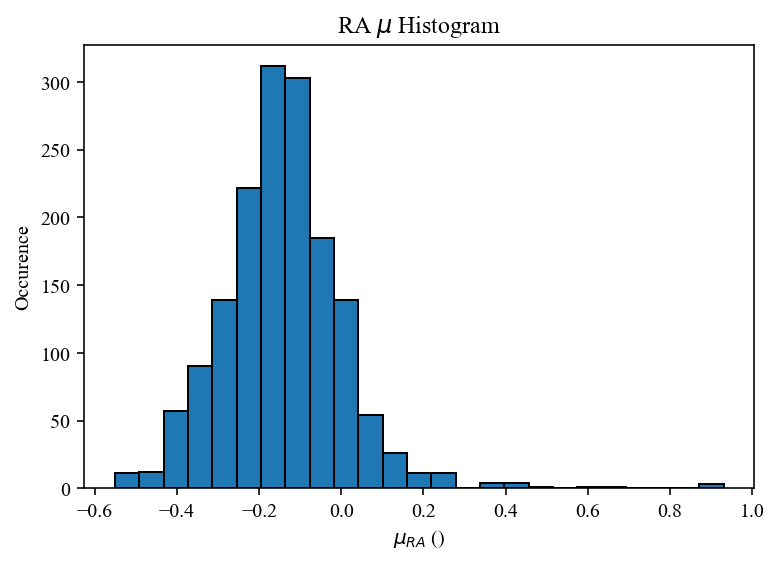
\includegraphics[scale = .5]{Figure 2025-02-08 230950 (2).png}
    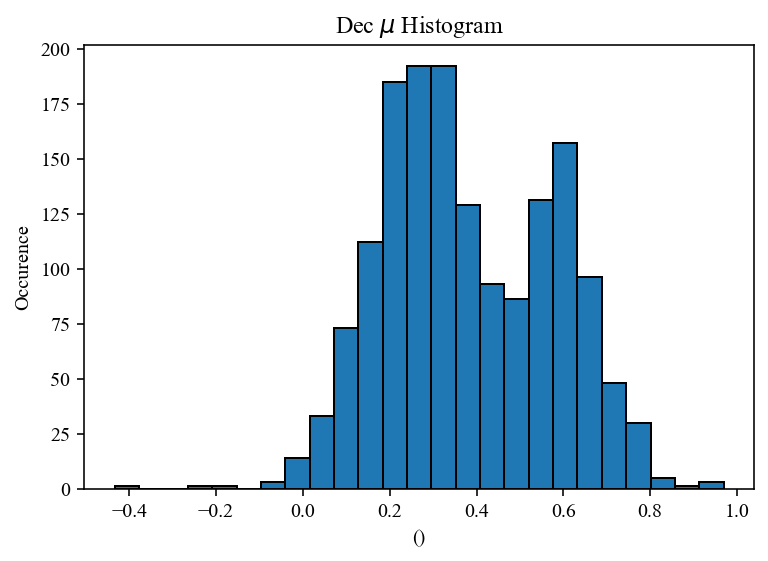
\includegraphics[scale = .5]{Figure 2025-02-08 230950 (3).png}
    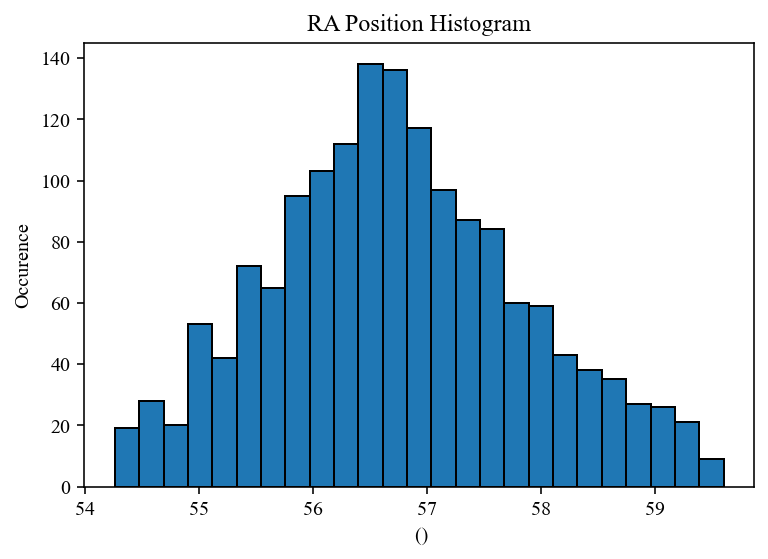
\includegraphics[scale = .5]{Figure 2025-02-08 230950 (4).png}
    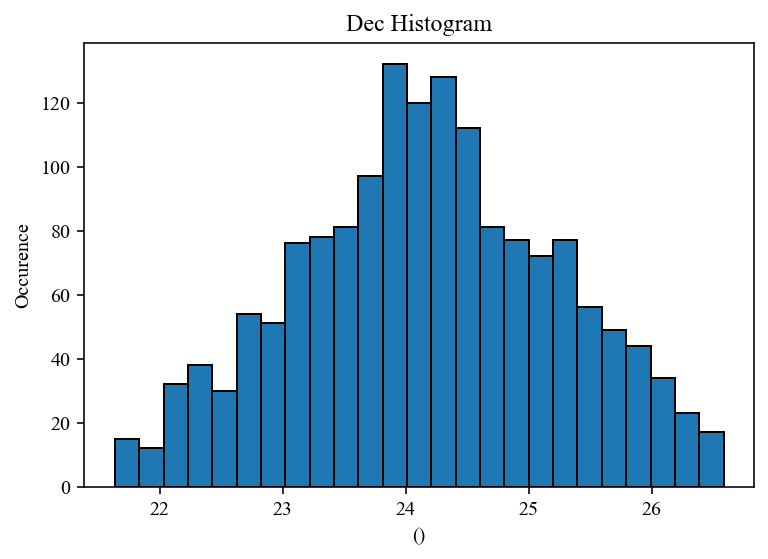
\includegraphics[scale = .5]{Figure 2025-02-08 230950 (5).png}
\end{figure}

Note, on the parallax histogram, we have extreme pollution from stars ranging from -2 ot 4 arcseconds.
The Pleiades, according to current NASA estimates, its distance of about 130 parsecs should mean it has parallax values of about 7 arcseconds.

\section{Cuts and Code}

\begin{python}
    # -*- coding: utf-8 -*-
    """
    Created on Fri Feb  7 11:43:44 2025

    @author: cmark
    """

    ## data import

    import pandas as pd
    import os 
    import matplotlib.pyplot as plt
    import numpy as np

    os.chdir("C:/Users/cmark/Spyder/PHSCS 428")

    data = pd.read_csv('Pleiades-result.csv')

    #%% plotting
    plt.rcParams['font.family'] = 'Times New Roman'

    plt.figure()
    plt.scatter(data['phot_bp_mean_mag'] - data['phot_rp_mean_mag'], data['phot_g_mean_mag'], s=.2, color='black')
    plt.xlabel("$G_{BP} - G_{RP}$")
    plt.ylabel("$G$")
    plt.show()

    #%% startng cuts

    ## from NASA, distance is 445 ly = 136.43 pc, which is about 7.4 arcsec

    plt.hist(data['parallax'], bins=25, range= (-5, 8), edgecolor='black')
    plt.title('$\pi$ Histogram')
    plt.xlabel('$\pi$ (arcsec)')
    plt.ylabel('Occurence')

    data_parallax = data[(data['parallax'] >= 6) & (data['parallax'] <= 8)]

    #%% RA Proper Motion

    plt.hist(data_parallax['ra_pmra_corr'], bins =25, edgecolor='black')
    plt.title('RA $\mu$ Histogram')
    plt.xlabel('$\mu_{RA}$ ()')
    plt.ylabel('Occurence')

    data_rapm= data_parallax[(data_parallax['ra_pmra_corr']>=-0.5) & (data_parallax['ra_pmra_corr'] <=.3)]
    #%% Dec Proper Motion

    plt.hist(data_parallax['dec_pmdec_corr'], bins =25, edgecolor='black')
    plt.title('Dec $\mu$ Histogram')
    plt.xlabel('()')
    plt.ylabel('Occurence')

    data_decpm = data_rapm[(data_rapm['dec_pmdec_corr'] >= -0.1) & (data_rapm['dec_pmdec_corr'] <= 0.9)]
    #%% Position

    plt.figure()
    plt.hist(data_parallax['ra'], bins =25, edgecolor='black')
    plt.title('RA Position Histogram')
    plt.xlabel(' ()')
    plt.ylabel('Occurence')
    plt.show() 

    plt.figure()
    plt.hist(data_parallax['dec'], bins =25, edgecolor='black')
    plt.title('Dec Histogram')
    plt.xlabel('()')
    plt.ylabel('Occurence')
    plt.show()

    data_pra = data_decpm[(data_decpm['ra'] >= 54.5) & (data_decpm['ra'] <= 58.5)]
    data_pdec = data_pra[(data_pra['dec'] >= 22) & (data_pra['dec'] <= 27)]

    #%% final CMD

    datafinal = data_pdec

    plt.figure()
    plt.title('Color Magnitude Diagram Final')
    plt.scatter(datafinal['phot_bp_mean_mag'] - datafinal['phot_rp_mean_mag'], datafinal['phot_g_mean_mag'], s=.2, color='black')
    plt.xlabel("$G_{BP} - G_{RP}$")
    plt.ylabel("$G$")
    plt.show()

    plt.figure()
    plt.title('Color Magnitude Diagram Combined')
    plt.scatter(data['phot_bp_mean_mag'] - data['phot_rp_mean_mag'], data['phot_g_mean_mag'], s=.2, color='black')
    plt.scatter(datafinal['phot_bp_mean_mag'] - datafinal['phot_rp_mean_mag'], datafinal['phot_g_mean_mag'], s=.2, color='red')
    plt.xlabel("$G_{BP} - G_{RP}$")
    plt.ylabel("$G$")
    plt.show()


    #%% vector plot

    plt.figure()
    plt.title('VPD')
    plt.scatter(data['ra_pmra_corr']*np.cos(data['dec_pmdec_corr']), data['dec_pmdec_corr'], s=.04)
    plt.xlabel('RA')
    plt.ylabel('Dec')
    plt.show()

    plt.figure()
    plt.title('VPD Final')
    plt.scatter(datafinal['ra_pmra_corr']*np.cos(datafinal['dec_pmdec_corr']), datafinal['dec_pmdec_corr'], s=.8)
    plt.xlabel('RA')
    plt.ylabel('Dec')
    plt.show()

    plt.figure()
    plt.title('VPD Combined')
    plt.scatter(data['ra_pmra_corr']*np.cos(data['dec_pmdec_corr']), data['dec_pmdec_corr'], s=.04)
    plt.scatter(datafinal['ra_pmra_corr']*np.cos(datafinal['dec_pmdec_corr']), datafinal['dec_pmdec_corr'], s=.8, color='red')
    plt.xlabel('RA')
    plt.ylabel('Dec')
    plt.show()

\end{python}

The cuts made are as follows:

\begin{center}
    \begin{tabular}{| c | c | c |}
        \hline
        Parameter & Minimum Value & Maximum Value \\
        \hline
        Parallax & -5 & 8\\
        Proper Motion (RA) & -0.5 & 0.3\\
        Proper Motion (Dec) & -0.1 & 0.9\\
        RA & 54.5 & 58.5\\
        Declination & 22 & 27\\
        \hline
    \end{tabular}
\end{center}

\section{Combined Plots}

The final data frame contained 1397 objects, which is 97 more than Heyl et al.
The final CMDs and VPDs are below.

\begin{figure}
    [H]
    \centering
    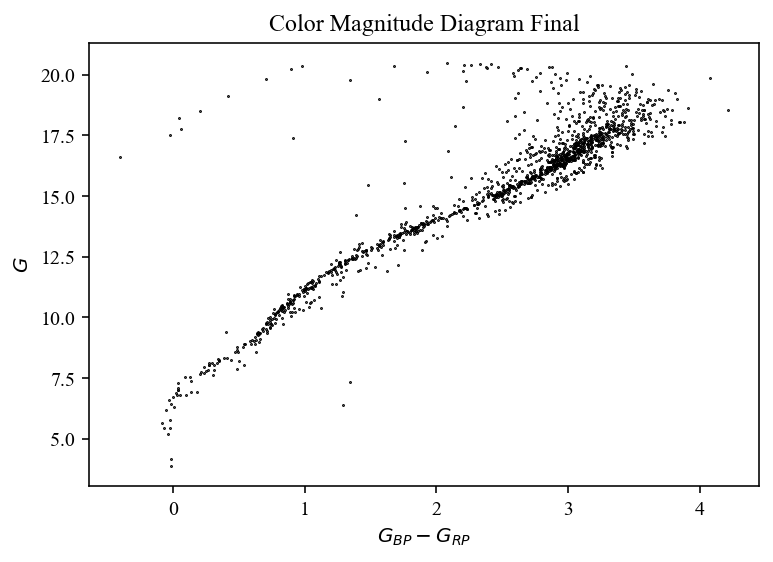
\includegraphics[scale = .5]{Figure 2025-02-08 230950 (6).png}
    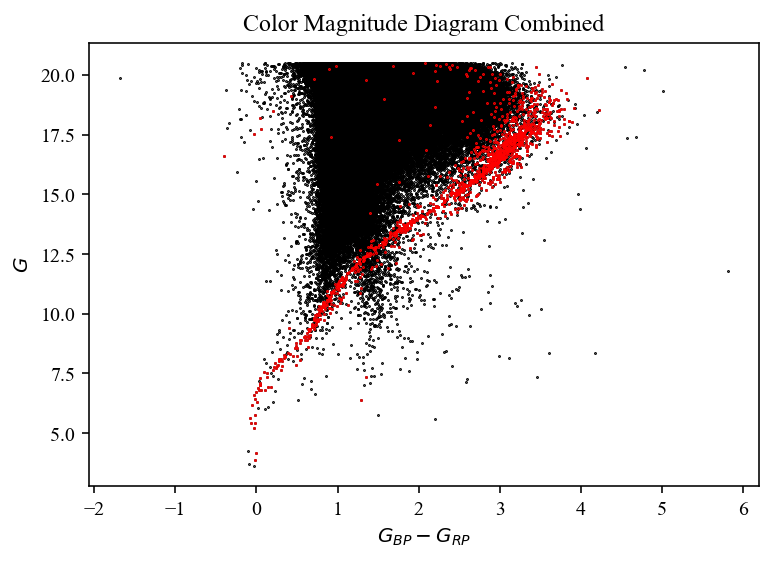
\includegraphics[scale = .5]{Figure 2025-02-08 230950 (7).png}
    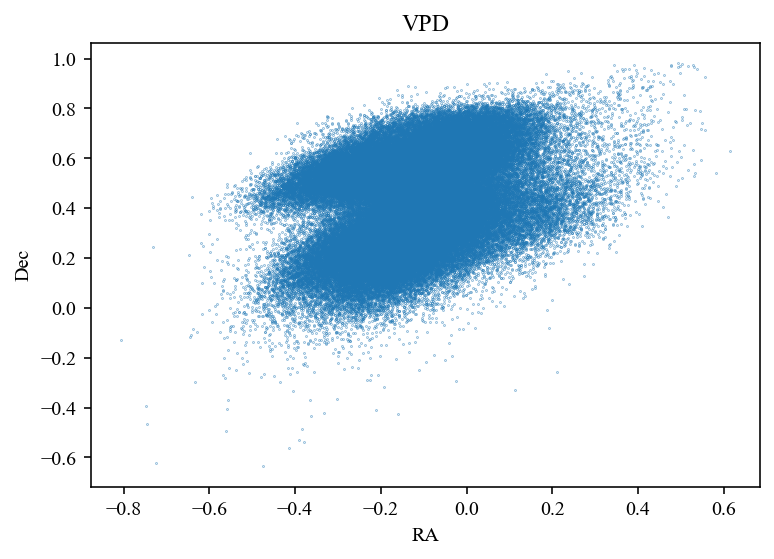
\includegraphics[scale = .5]{Figure 2025-02-08 230950 (8).png}
    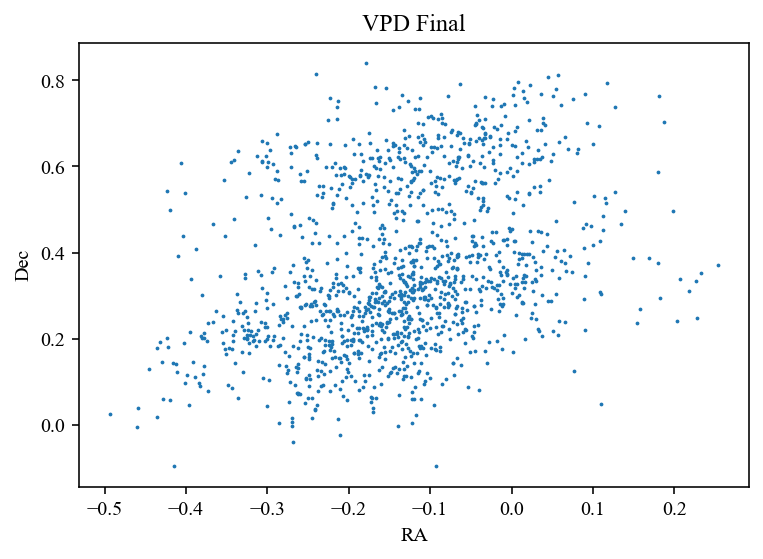
\includegraphics[scale = .5]{Figure 2025-02-08 230950 (9).png}
    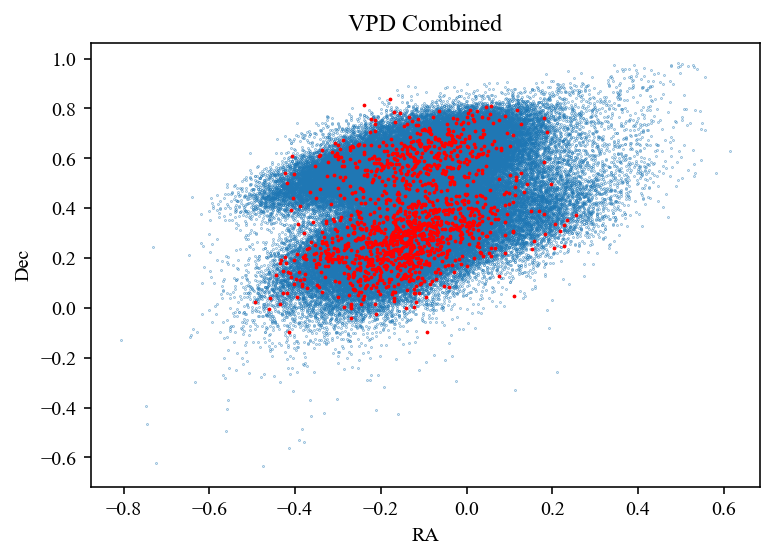
\includegraphics[scale = .5]{Figure 2025-02-08 230950 (10).png}
\end{figure}

After rejection, we obtain an average distance value of:
7.217 $mas$. This corresponds to a distance of about 138 parsec.


\begin{python}
    #%%

    average = datafinal['parallax'].mean()
    print(f"Average value: {average}")
    distance = 1/average
    print(f"Calculated Distance: {distance}")
\end{python}
\end{document}